%!TEX root = ../TAMUTemplate.tex
%%%%%%%%%%%%%%%%%%%%%%%%%%%%%%%%%%%%%%%%%%%%%%%%%%%
%
%  New template code for TAMU Theses and Dissertations starting Fall 2016.
%
%  Author: Sean Zachary Roberson
%	 Version 3.16.09
%  Last updated 9/12/2016
%
%%%%%%%%%%%%%%%%%%%%%%%%%%%%%%%%%%%%%%%%%%%%%%%%%%%
%%%%%%%%%%%%%%%%%%%%%%%%%%%%%%%%%%%%%%%%%%%%%%%%%%%%%%%%%%%%%%%%%%%%%%
%%                           SECTION VI
%%%%%%%%%%%%%%%%%%%%%%%%%%%%%%%%%%%%%%%%%%%%%%%%%%%%%%%%%%%%%%%%%%%%%


\chapter{\texorpdfstring{\uppercase {Results}}{Results}}
\label{ch:results}

\begin{figure}[!hbtp]
    \centering
    \begin{subfigure}[t]{0.316\textwidth}
        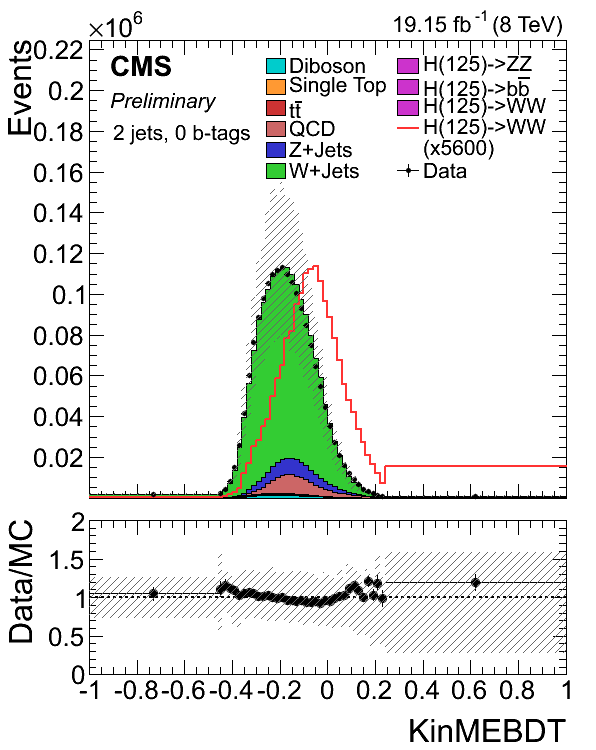
\includegraphics[width=\textwidth]{\figpath/Chapter6/KinMEBDT_jets2_electron.png}
        \caption{}
        \label{fig:KinMEBDT_jets2_electron}
    \end{subfigure}
    \begin{subfigure}[t]{0.316\textwidth}
        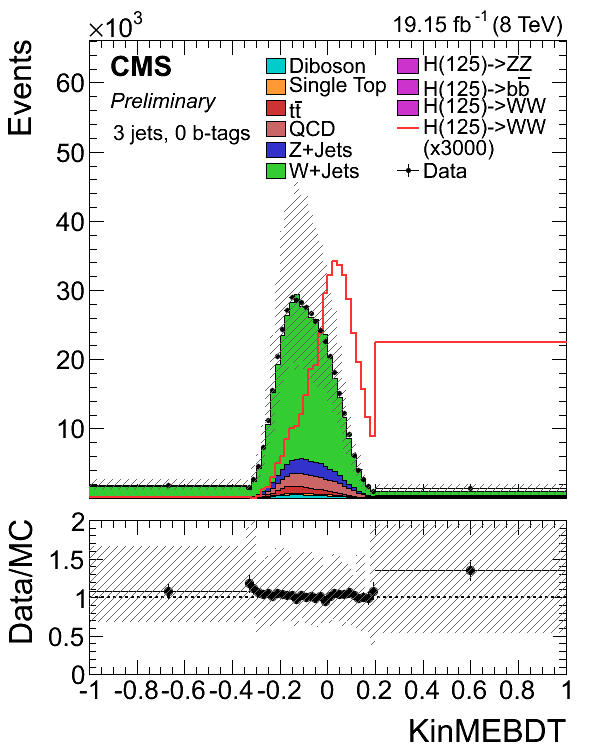
\includegraphics[width=\textwidth]{\figpath/Chapter6/KinMEBDT_jets3_electron.png}
        \caption{}
        \label{fig:KinMEBDT_jets3_electron}
    \end{subfigure}
    \begin{subfigure}[t]{0.316\textwidth}
        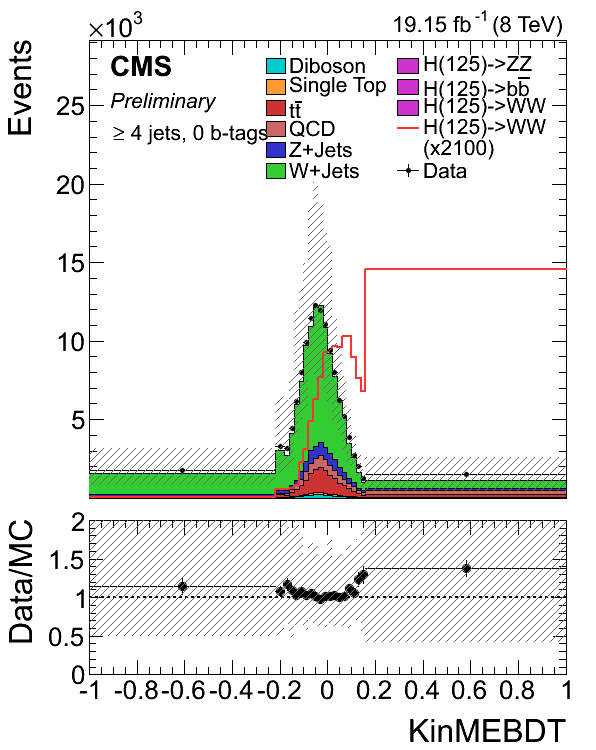
\includegraphics[width=\textwidth]{\figpath/Chapter6/KinMEBDT_jets4_electron.png}
        \caption{}
        \label{fig:KinMEBDT_jets4_electron}
    \end{subfigure}

    \begin{subfigure}[t]{0.316\textwidth}
        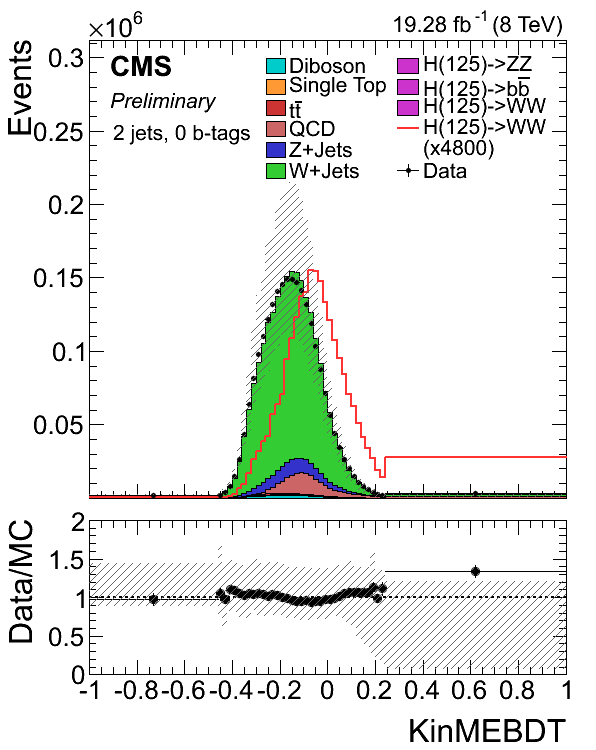
\includegraphics[width=\textwidth]{\figpath/Chapter6/KinMEBDT_jets2_muon.png}
        \caption{}
        \label{fig:KinMEBDT_jets2_muon}
    \end{subfigure}
    \begin{subfigure}[t]{0.316\textwidth}
        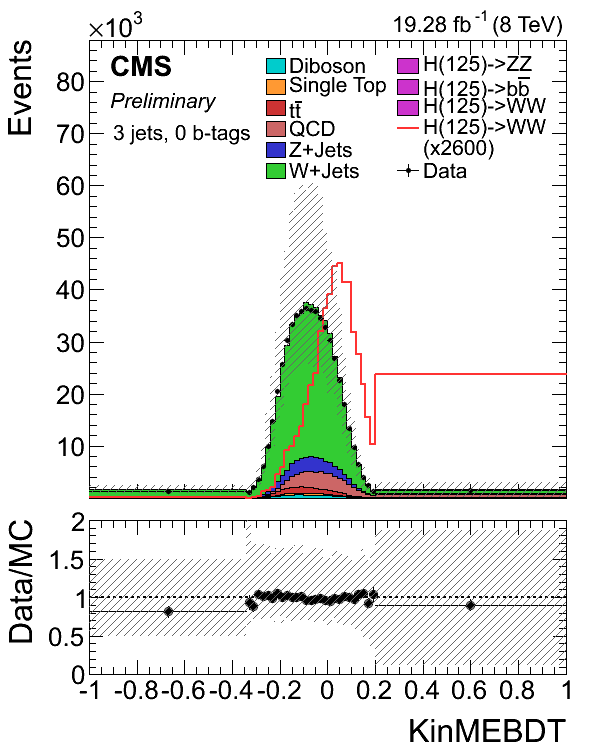
\includegraphics[width=\textwidth]{\figpath/Chapter6/KinMEBDT_jets3_muon.png}
        \caption{}
        \label{fig:KinMEBDT_jets3_muon}
    \end{subfigure}
    \begin{subfigure}[t]{0.316\textwidth}
        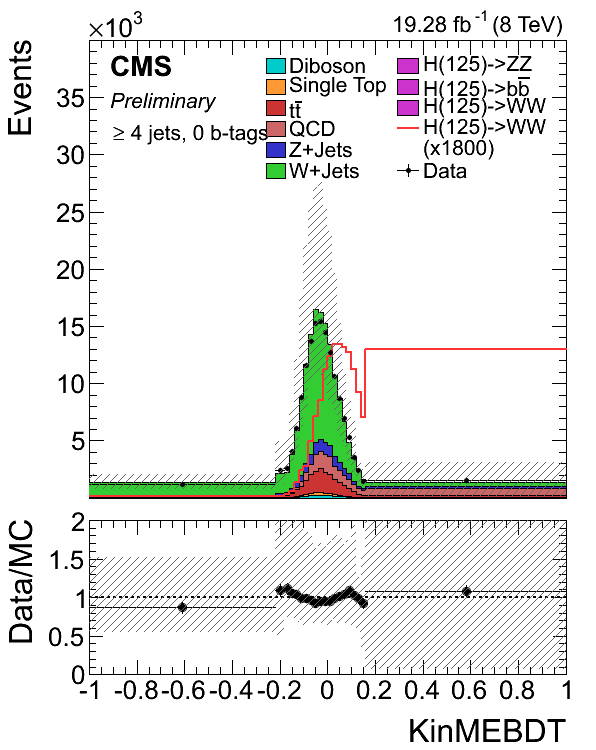
\includegraphics[width=\textwidth]{\figpath/Chapter6/KinMEBDT_jets4_muon.png}
        \caption{}
        \label{fig:KinMEBDT_jets4_muon}
    \end{subfigure}
    \caption{The KinMEBDT distribution in Monte Carlo (filled histograms) and data (black markers). The \HWW signal is shown by red line while the systematic uncertainties are shown by the hashed areas. The plots are ordered by jet bin from left to right, with the leftmost plot being the two-jet bin and the rightmost plot being the greater than or equal to four-jet bin. The top row contains the electron channel plots while the bottom rows contain the muon channel plots.}
    \label{fig:KinMEBDT_final_templates}
\end{figure}

\begin{figure}[!hbt]
    \centering
    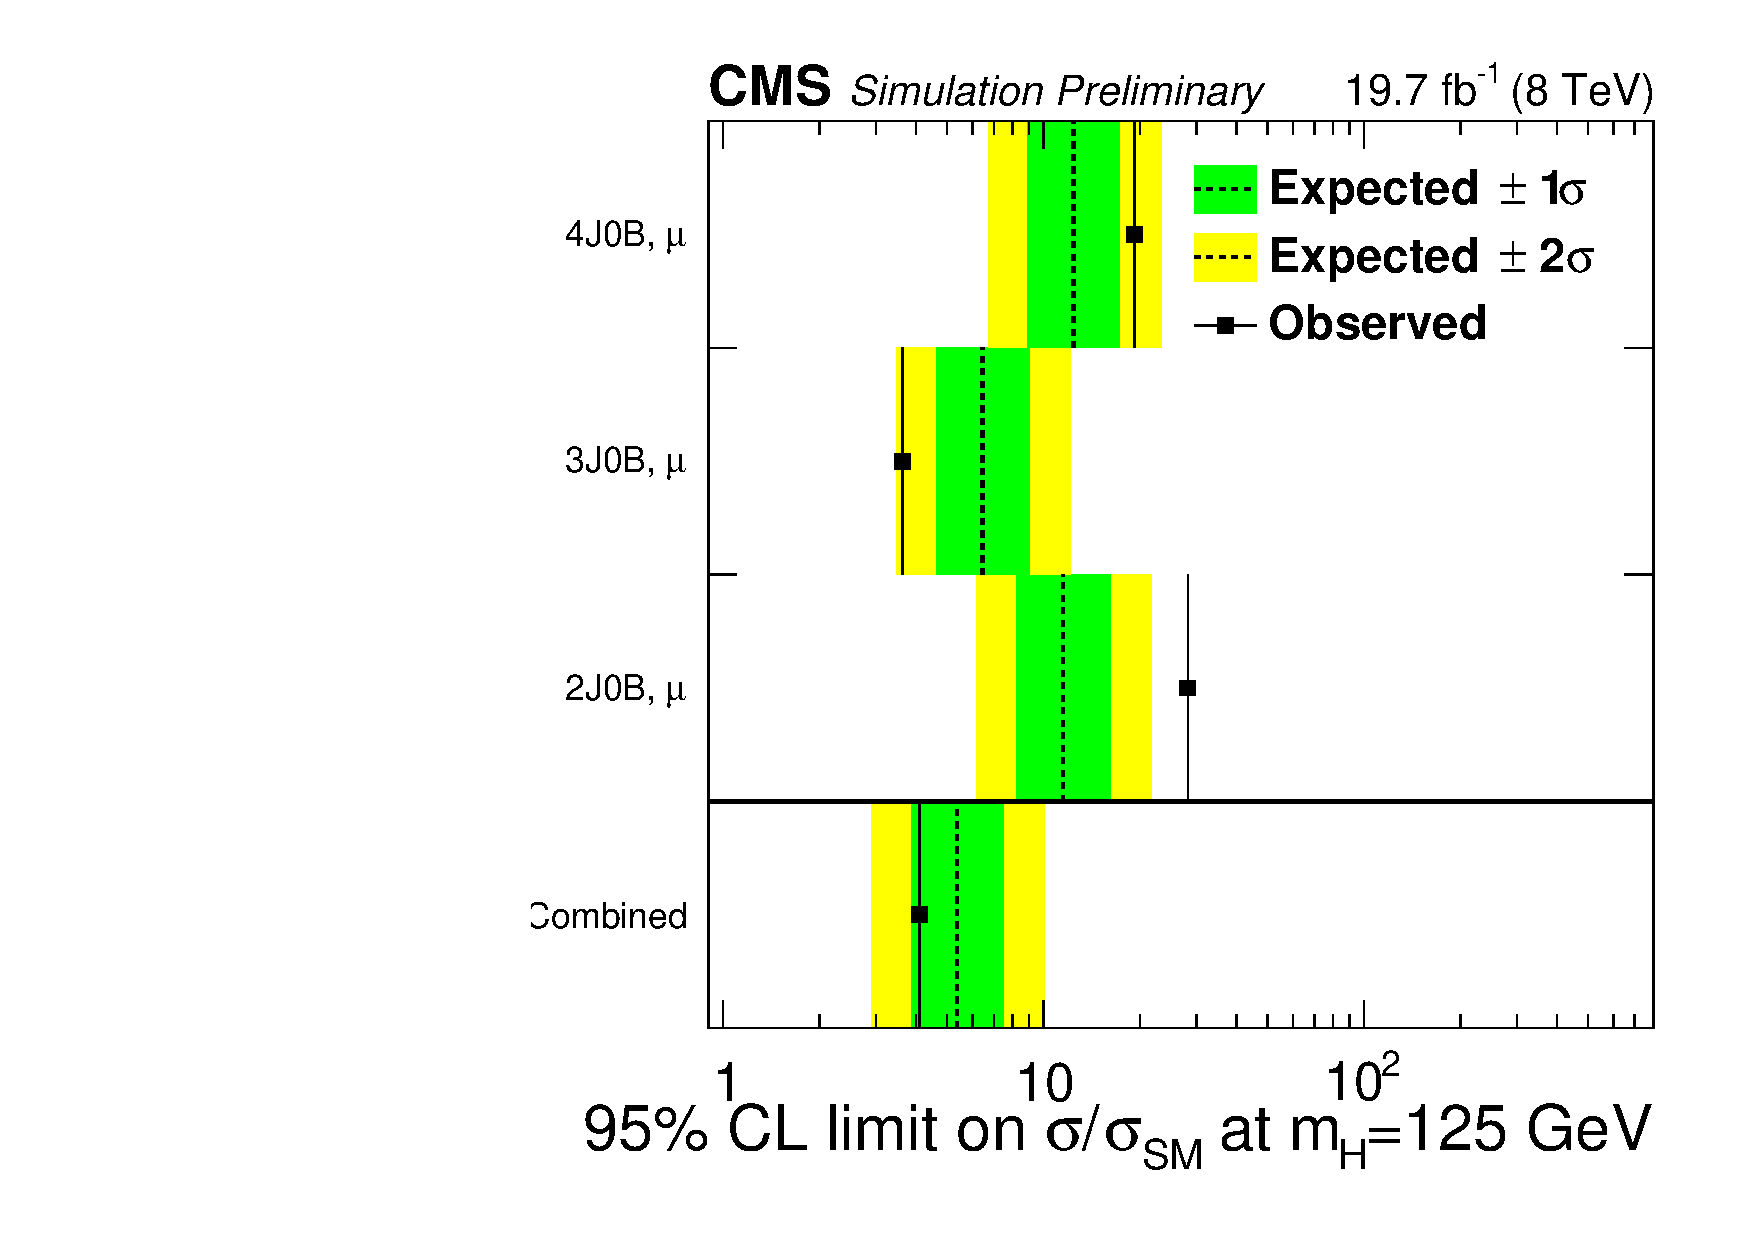
\includegraphics[width=0.95\textwidth]{\figpath/Chapter6/2017_10_05_combinedSM_KinMEBDT_muon.pdf}
    \caption{Expected 95\% upper confidence level on the Higgs signal strength for only the muon channel.}
    \label{fig:limits_withSys_muon}
\end{figure}


\begin{table}[htbp]
\centering
\begin{tabular}{lrrr|r} \hline
Lepton Channel      & 2 Jets  & 3 Jets  & $\geqslant$4 Jets & Combined Jet \\\hline
Electron            &         &         &                   &              \\
Muon                &         &         &                   &              \\\hline
Combined Lepton     &         &         &                   &              \\\hline
\end{tabular}
\caption{}
\label{tab:95percent_upper_confidence_levels}
\end{table}


\begin{comment}
A distribution of the BDT discriminant is produced for every signal, background, and data sample and then passed to the RooStats-based Higgs Combine Tool~\cite{CombineToolTwiki} to compute limits on the Higgs signal strength.
Given that this analysis has a relatively high number of events in the expected yields we make use of the asymptotic method\footnote{If there had been a lower number of expected events we may have needed to use the full frequentist method rather than the asymptotic method.} for limit setting along with the CL\textsubscript{s} test statistic~\cite{Read:2002hq}.
Using an Asimov dataset an expected 95\% upper confidence level is obtained and shown in figure~\ref{fig:limits} (left).


original bin width 0.02 [-1,1]
bin must have background events
stat error must be less than 10\%
bins merged left to right until all bins meet this criteria
limited or no background in a bin would lead to an inflated signal significance if data, but no background


effect on the limit calculation if that uncertainty is removed from the calculation.


begin{figure}[!hbt]
	\centering
	\begin{subfigure}[t]{0.46\textwidth}
		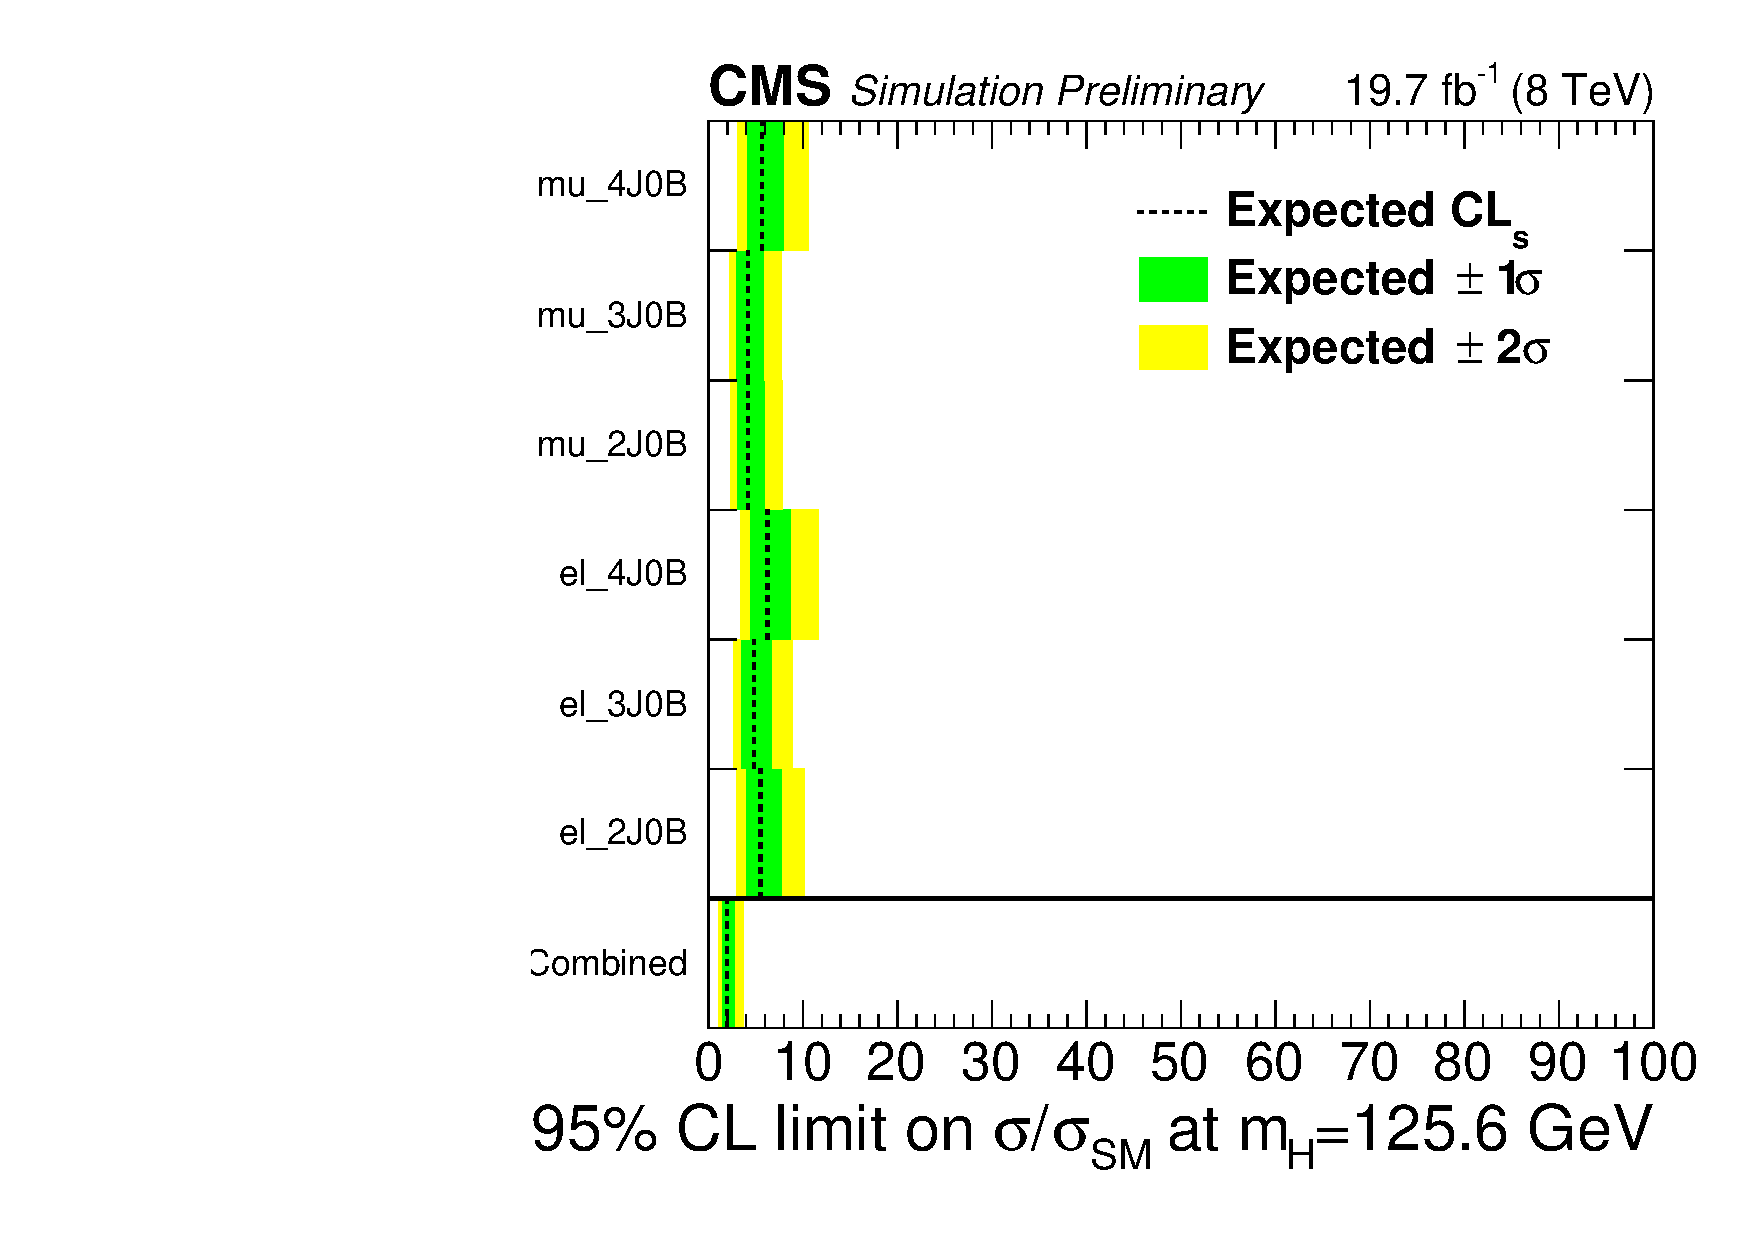
\includegraphics[width=\textwidth]{\figpath/Chapter4/2015_08_01_combinedSM_KinMEBDT_StatsOnly.pdf}
		\label{fig:limits_stats_only}
	\end{subfigure}
	\begin{subfigure}[t]{0.46\textwidth}
		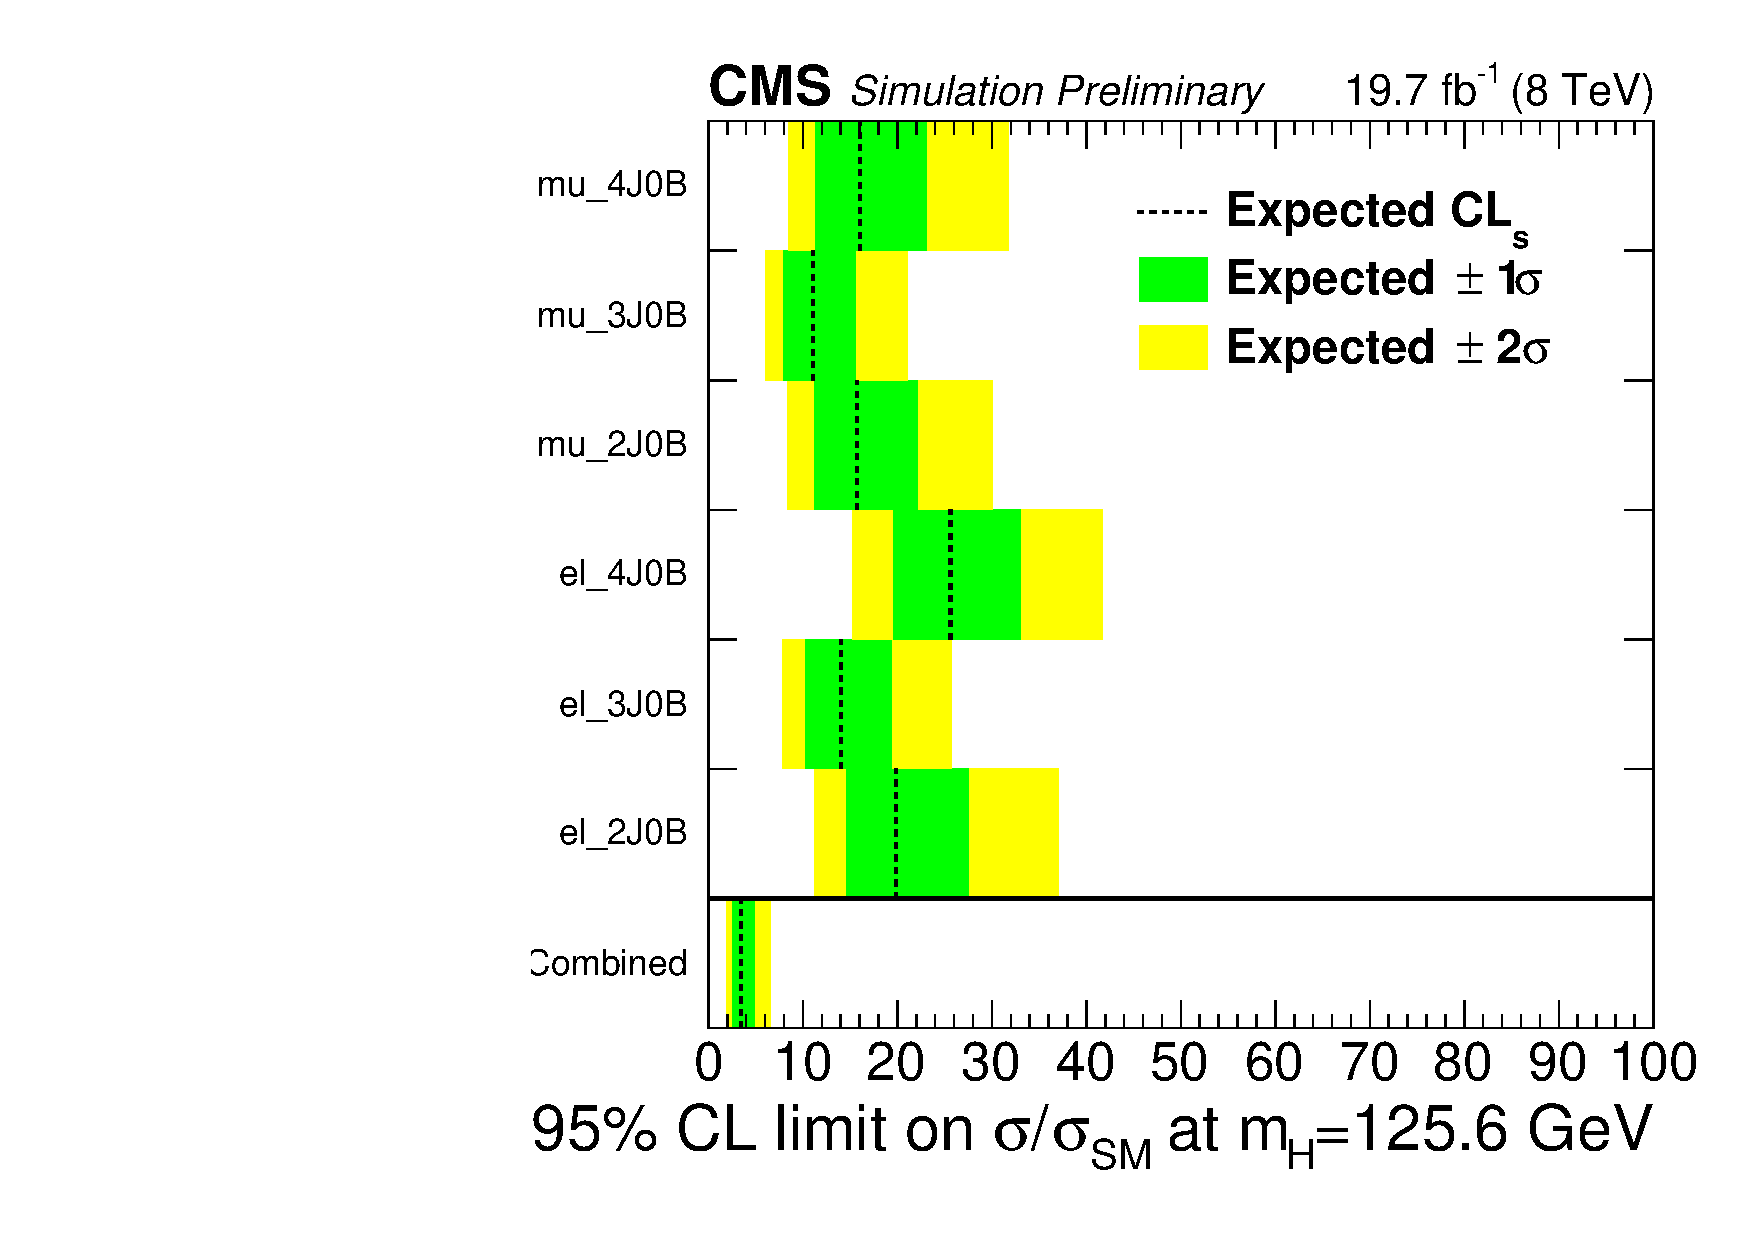
\includegraphics[width=\textwidth]{\figpath/Chapter4/2015_08_01_combinedSM_KinMEBDT.pdf}
		\label{fig:limits_with_sys}
	\end{subfigure}
	\caption{Expected 95\% upper confidence level on the Higgs signal strength (left) without including systematic uncertainties and (right) with systematic uncertainties included. The median combined limit is found to be 2.01 without systematics and 3.48 with them.}
	\label{fig:limits}
\end{figure}
\end{comment}